\documentclass[10pt,a4paper]{article}

%%%%%%%%%%%%%%%%%%%%%%%%%%%
% MODIFY:

\newcommand{\authorA}{ALEX PASQUALI (03754113)}
\newcommand{\authorB}{NICOLA GUGOLE (03753996)}
\newcommand{\groupNumber}{A} % - YOUR GROUP NUMBER
\newcommand{\exerciseNumber}{1} % - THE NUMBER OF THE EXERCISE
\newcommand{\sourceCodeLink}{https://github.com/AlexPasqua/MLCMS-exercises}

\newcommand{\workPerAuthor}{
\authorA&Task 1&50\%\\
      &Task 2&50\%\\
      &Task 3&50\%\\
      &Task 4&50\%\\
      &Task 5&50\%\\
      \hline
\authorB&Task 1&50\%\\
      &Task 2&50\%\\
      &Task 3&50\%\\
      &Task 4&50\%\\
      &Task 5&50\%\\
      \hline
}

%%%%%%%%%%%%%%%%%%%%%%%%%%%

%%
% imports for the exercise sheets
%

\usepackage[utf8]{inputenc}
\usepackage{amsmath}
\usepackage{amsfonts}
\usepackage{amssymb}

\usepackage[yyyymmdd]{datetime}
\renewcommand{\dateseparator}{--}

\usepackage[left=2cm,right=2cm,top=3cm,bottom=3cm]{geometry}

\usepackage{hyperref}

\usepackage{amsthm}
\newtheorem{lem}{Lemma}
\newtheorem{thm}{Theorem}
\newtheorem{cor}{Corollary}
\newtheorem{rem}{Remark}
\newtheorem{definition}{Definition}
\newtheorem{ter}{Terminology}

\usepackage{graphicx}

\newcommand{\M}{\mathcal{M}}
\newcommand{\N}{\mathcal{N}}
\newcommand{\K}{\mathcal{K}}
\newcommand{\SPDk}{\mathbb{P}^k}
\newcommand{\vol}{\text{vol}}

\newcommand{\Figref}[1]{Figure~\ref{#1}}
\newcommand{\figref}[1]{figure~\ref{#1}}
\newcommand{\Eqnref}[1]{Equation~(\eqref{#1})}
\newcommand{\eqnref}[1]{equation~(\eqref{#1})}

\usepackage{float}
\usepackage{tabularx}

\usepackage{fancyhdr}
\pagestyle{fancy}

\usepackage{totcount}
\newtotcounter{taskCounter}
\newtotcounter{pointCounter}
\newenvironment{task}[1]{\noindent\stepcounter{taskCounter}\textbf{Report on task #1}\smallbreak\hrule\smallbreak}{\smallbreak\hrule\bigbreak}


\title{Report for exercise \exerciseNumber~from group~\groupNumber}

\makeatletter
\let\thetitle\@title
\let\theauthor\@author
\let\thedate\@date
\makeatother

\providecommand{\versiondate}{\today}

\lhead{Exercise sheet \exerciseNumber}
\chead{Master Praktikum: Modelling and Simulation of Crowds WS2019/20}
\rhead{TUM}
\lfoot{Report of Group \groupNumber}
\cfoot{\thepage}
\rfoot{Last compiled: \versiondate}
\renewcommand{\headrulewidth}{0.4pt}
\renewcommand{\footrulewidth}{0.4pt}

\newcommand{\frontpage}{
\begin{center}
\textbf{\thetitle}\\~\\
\end{center}
\begin{table}[H]
\begin{tabular}{ll}
Tasks addressed:&\total{taskCounter}\\
Authors:&\authorA\\
&\authorB\\
&\authorC\\
Last compiled:&\versiondate\\
Source code:&\sourceCodeLink
\end{tabular}
\end{table}
\vfill
The work on tasks was divided in the following way:
\begin{table}[H]
\begin{tabularx}{\textwidth}{X|p{2cm}|p{2cm}}
\workPerAuthor
\end{tabularx}
\end{table}
\newpage
}
\graphicspath{ {images/} }

\begin{document}

\frontpage

\begin{task}{1, Setting up the modeling environment}
\paragraph{High level description}
First of all, a graphical visualization of the environment was created.
It consists of a squared grid and it is possible to specify the size, as well as the length of the side of each cell.
This was practically implemented in Python, using the \texttt{tkinter} package for the graphical aspects of the project.

\begin{figure}[H]
    \centering
    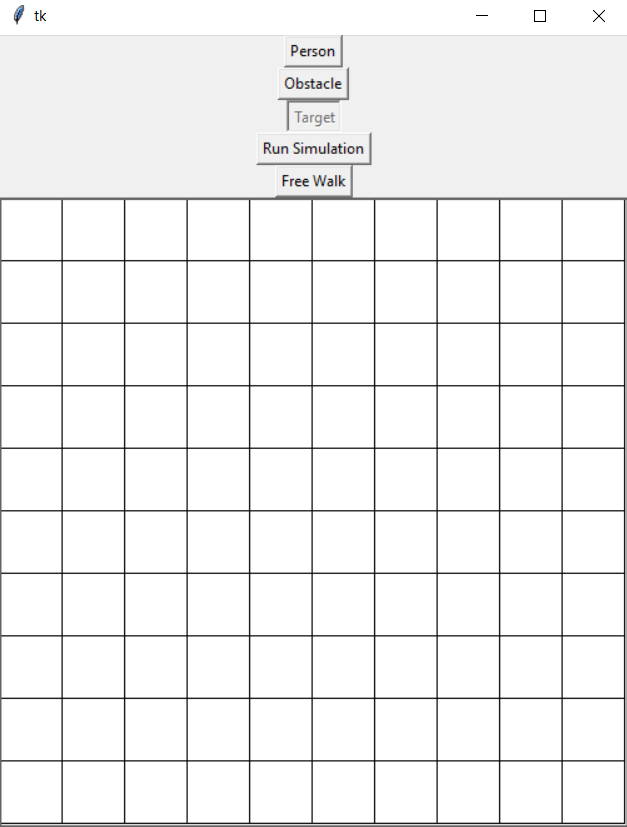
\includegraphics[scale=0.5]{empty_grid.png}
    \caption{Empty grid with some selection buttons}
    \label{fig:empty-grid}
\end{figure}

It is possible to insert elements in the environment through the selection buttons on top of the grid (\hyperref[fig:empty-grid]{Fig. \ref{fig:empty-grid}}):
first click on the button representing the desired object (person (in red) / obstacle (in black) / target (in green)) and then click the cells to be filled with that object.
It is possible to remove or convert an object by simply clicking again on an occupied cell.

The \texttt{Free Walk} mode makes possible to select a pedestrian - by clicking on it - and move it with the 4 arrows buttons on the keyboard.
Stepping on a target will make the pedestrian disappear (\textit{absorbent targets}) and the cells occupied by obstacles and other pedestrians are not accessible.
After clicking on the \texttt{Free Walk} button, it changes its descriptive text to \texttt{Editing mode}, that, when selected, brings back the possibility of modifying the environment, adding objects or changing their disposition.

The \texttt{Simulation} mode starts to simulate the behavior of the pedestrian, who try to reach the \textit{nearest target} in the quickest way possible.
In turns, each pedestrian update its cost matrix, which has a size of 3x3 where every element represent the cost function's value of moving to any one of the neighbor cells.
This value corresponds to the euclidean distance between that cell and the nearest target.
The cost for all the cells occupied by obstacles or other pedestrian is set to infinity (using Python's \texttt{math.inf}).
Having this information, the pedestrian plans the move to make and sets the destination cell as occupied in the \textit{planning grid}
\footnote{A copy of the grid where the planned moves by pedestrians are executed immediately. This way, other pedestrians, when planning their own move, will know that some cells will be occupied, thus inaccessible.}.
Subsequently, according to the type of move - if diagonal or along the cardinal axes - the pedestrian's waiting time is set respectively to 1.4 and 1.0 seconds
\footnote{A diagonal move actually covers more space than one along the axes, therefore, assuming a fixed walking speed, it will take more time to be completed.}
to simulate a certain fixed walking speed.
Only when the waiting time is expired, the pedestrian will finally be allowed to move in the cell planned before.

The cellular automata update is not parallel but sequential. The fictitious parallelism is achieved by making all the pedestrians plan/execute move one by one (the choosing order is randomized at every cycle so to preserve equality and avoid advantaging a particular pedestrian) before updating the graphic application. A discretization of time is therefore fundamental, waiting a certain time step (by default 0.1s) between two updates so to simulate the time passing.

\paragraph{Code and implementation}
The whole project is implemented in Python (vers. 3.8) and \texttt{tkinter} \cite{tkinter} (vers. 8.6) is used to manage the graphical aspects.\\
The 3 main objects are: \textit{grid}, \textit{cell} and \textit{pedestrian}.
The \textbf{grid} is implemented through a class inheriting from tkinter's \texttt{Canvas}.
Its main attributes are:
\begin{itemize}
    \item \texttt{pedestrian\_list}: a list containing all the \texttt{Pedestrian} objects currently present on the grid.
    \item \texttt{pedestrian\_cell\_list}: list containing all the \texttt{Cell} objects currently occupied by a \textit{pedestrian}.
    \item \texttt{targets\_cell\_list}: list containing all the \texttt{Cell} objects currently occupied by a \textit{target}.
    \item \texttt{obstacles\_cell\_list}: list containing all the \texttt{Cell} objects currently occupied by an \textit{obstacle}.
\end{itemize}
All the commands are managed by some \textit{handler methods} and the grid also implements the actual simulation through a cycle contained in the apposite method \texttt{start\_simulation} (\hyperref[fig:simulation-cycle]{Fig. \ref{fig:simulation-cycle}}).
\begin{figure}[H]
    \centering
    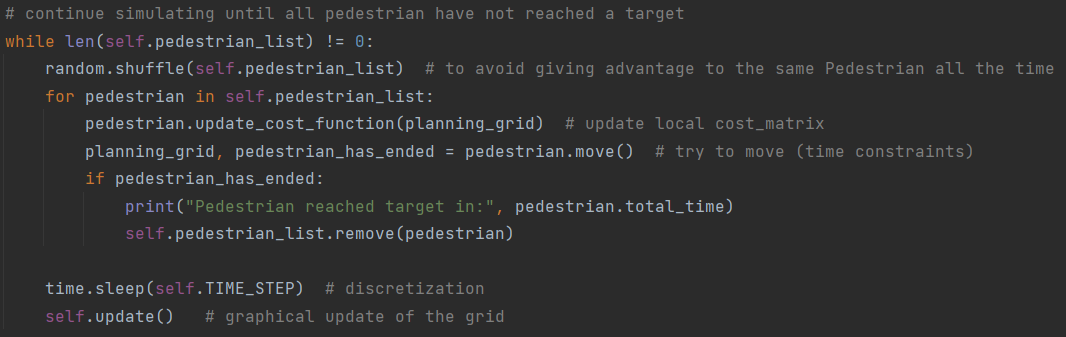
\includegraphics[scale=0.7]{simulation_cycle.png}
    \caption{Main cycle in \texttt{Grid}'s \texttt{start\_simulation} method}
    \label{fig:simulation-cycle}
\end{figure}

The \textbf{cell} is implemented through a class representing a single cell in the grid.
It has a \textit{status} (empty / pedestrian / obstacle / target) that is used to set its color and to instruct the grid about the presence of a specific object, by adding or removing elements to the grid's specific lists (\texttt{pedestrian\_cell\_list}, \texttt{targets\_cell\_list}, \texttt{obstacles\_cell\_list}).
This is useful to mask out the complexity of managing different status and situations: whenever the \texttt{draw} method is called, the cell will be colored correctly.

Finally, the \texttt{Pedestrian} class implements all the pedestrians' behaviors.
Its main methods are:
\begin{itemize}
    \item \texttt{update\_cost\_function (prior to Dijsktra)}:
    \begin{itemize}
        \item Finds the nearest target to the current pedestrian
        \item Updates its cost function (every pedestrian has its own cost function that changes depending of which one is the nearest target) depending on the euclidean distance between the pedestrian and said target
        \item Sets targets' cost to 0
        \item Sets obstacles and other pedestrians' costs to infinity
    \end{itemize}
    \item \texttt{plan\_move}: checks the costs of the neighbor cells and decides where to go next (cell with the lowest cost)
    \item \texttt{actuate\_move}: it actually makes the move in the planning or actual grid (depending on an argument passed to the method)
    \item \texttt{move}: after updating the cost function, this method is called in the main simulation cycle. It executes the following steps:
    \begin{itemize}
        \item if the pedestrian is active:
        \begin{itemize}
            \item Plans the next move (through \texttt{plan\_move})
            \item Executes the moves in the planning grid (through \texttt{actuate\_move})
            \item Sets the correct waiting time (i.e. the necessary time to cover one step - diagonal or cardinal)
            \item Sets itself as \textbf{not} active
        \end{itemize}
        \item otherwise: decrease the waiting time and if it comes to 0, actuates the move in the actual grid.
    \end{itemize}
\end{itemize}
\end{task}


\begin{task}{2, First step of a single pedestrian}
Task 2 consists of having a pedestrian 20 cells away from a target, respectively, they are located in (5, 25) and (25, 25).\\
By executing this task on the Jupyter notebook, a grid will be created representing exactly the scenario in object, and, by pressing the button \texttt{Run Simulation} (located on top of the grid) it will be possible to see the pedestrian walking in a straight line towards the target at a fixed speed (see \hyperref[fig:task2]{Figure \ref{fig:task2}} for some screenshot of the simulation).
Specifically, each cell has a side of 1 meter and the walking speed of the pedestrian is 1m/s, therefore, each step along the cardinal axes is going to cover 1 meter and take 1 second to be accomplished, while each diagonal step is going to cover 1.4 meters in 1.4 seconds.\\\\
\underline{As expected, in the experiments the pedestrian reaches the target in \textbf{20 seconds}.}\\\\
Note: the target is absorbent, therefore, when the pedestrian reaches the destination, it disappears.

\begin{figure}[H]
    \centering
    \subfloat[a]{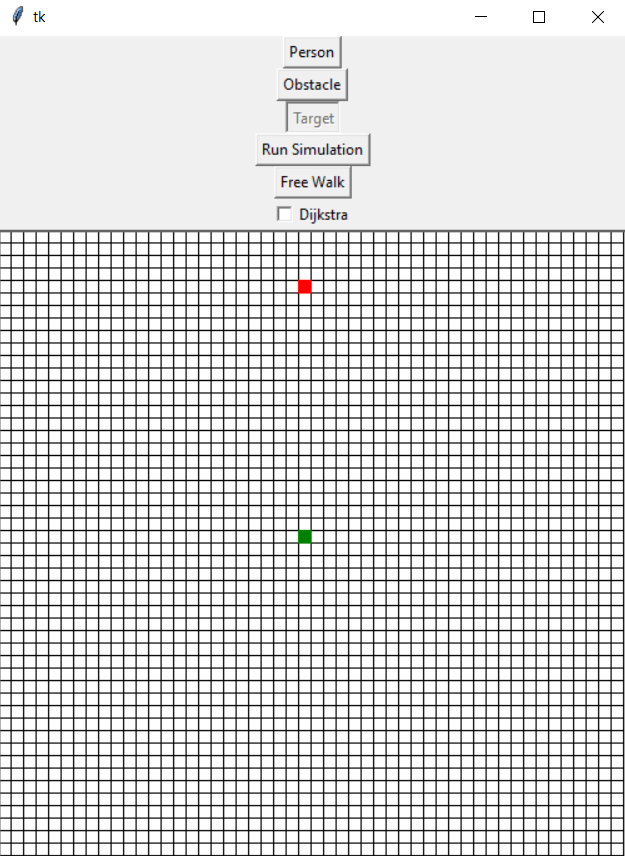
\includegraphics[width=0.3\textwidth]{task2_1.png}\label{fig:task2-1}}
    \hfill
    \subfloat[b]{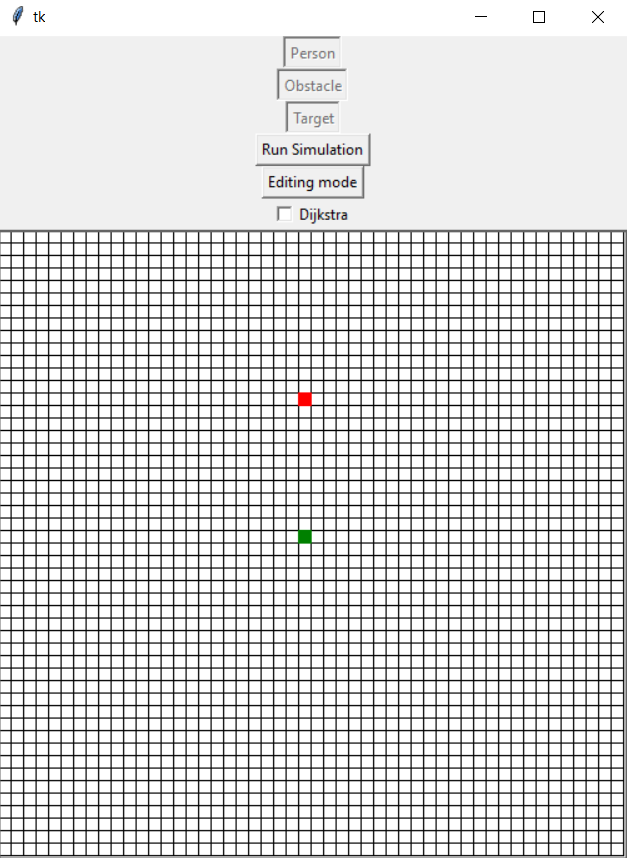
\includegraphics[width=0.3\textwidth]{task2_2.png}\label{fig:task2-2}}
    \hfill
    \subfloat[c]{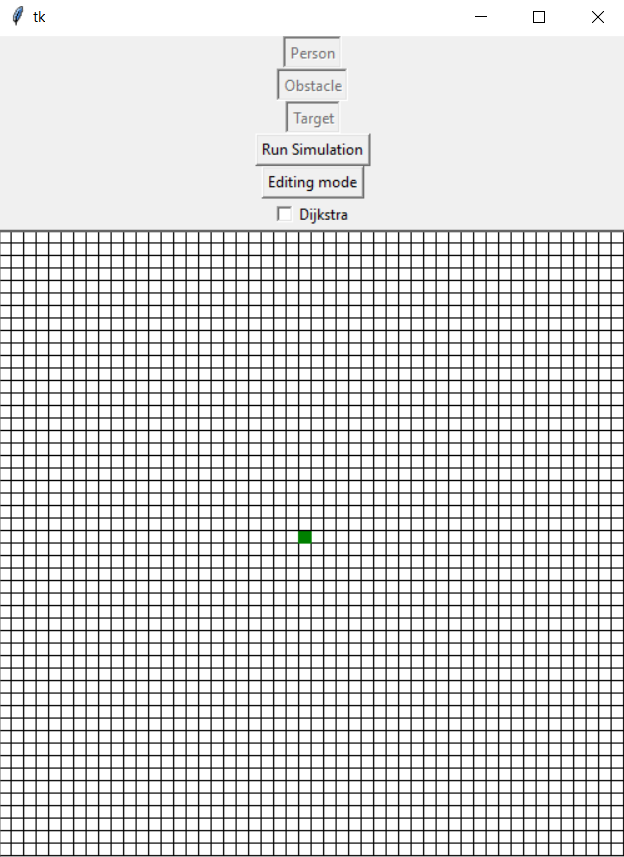
\includegraphics[width=0.3\textwidth]{task2_3.png}\label{fig:task2-3}}
    \caption{Screenshots showing 3 different stages of the task 2. The sub-figure (a) shows the initial setup; sub-figure (b) shows the environment in the middle of the simulation; sub-figure (c) shows the end on the simulation, when the pedestrian reached the target and has been absorbed.}
    \label{fig:task2}
\end{figure}
\end{task}


\begin{task}{3, Interaction of pedestrians}
This task consists of displaying a target in the center of the grid and 5 pedestrians around it, at the same distance (\hyperref[fig:task3]{Figure \ref{fig:task3}.a}).\\
Through the Jupyter notebook, it is possible to set up the scenario and start the graphical interface, on which, by clicking the apposite button, it is possible to run the simulation.
\hyperref[fig:task3]{Figure \ref{fig:task3}} shows 3 stages of the simulation.\\
Note that the goal of the pedestrians is to "step" on the target, and when they do so, they get \textit{absorbed}.\\\\
In the experiments, all pedestrians have been placed at roughly
\footnote{The discretization of the space does not always allow to place pedestrian at the \textbf{exact} desired distance.}
\textbf{21 meters distance} from the target and they all reach the target after \textbf{21 seconds} of simulation.\\

\begin{figure}[H]
    \centering
    \subfloat[a]{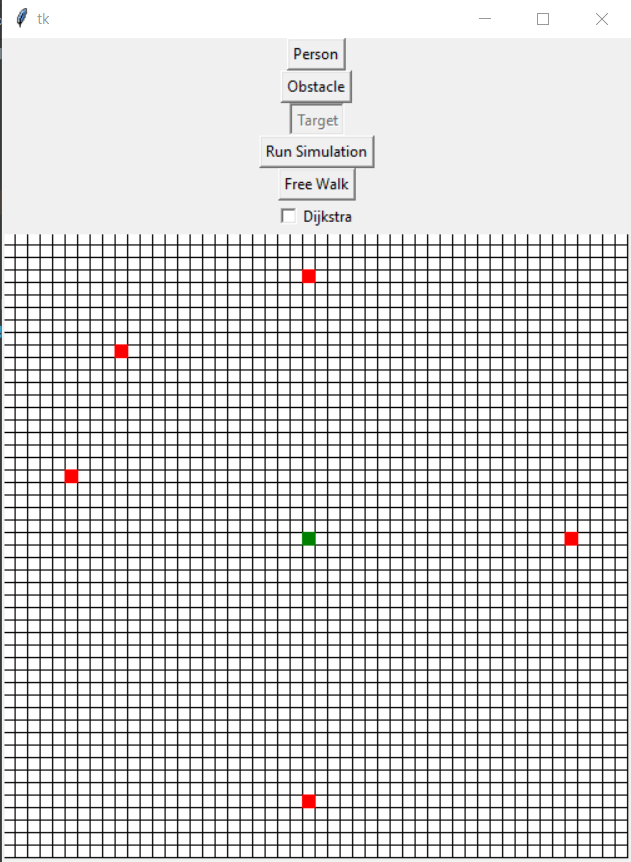
\includegraphics[width=0.3\textwidth]{task3_1.png}\label{fig:task3-1}}
    \hfill
    \subfloat[b]{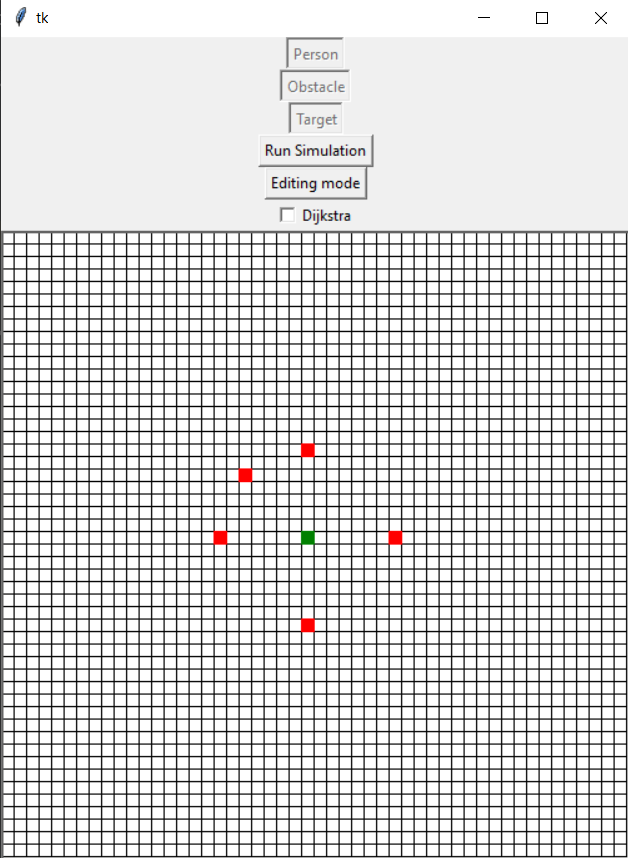
\includegraphics[width=0.3\textwidth]{task3_2.png}\label{fig:task3-2}}
    \hfill
    \subfloat[c]{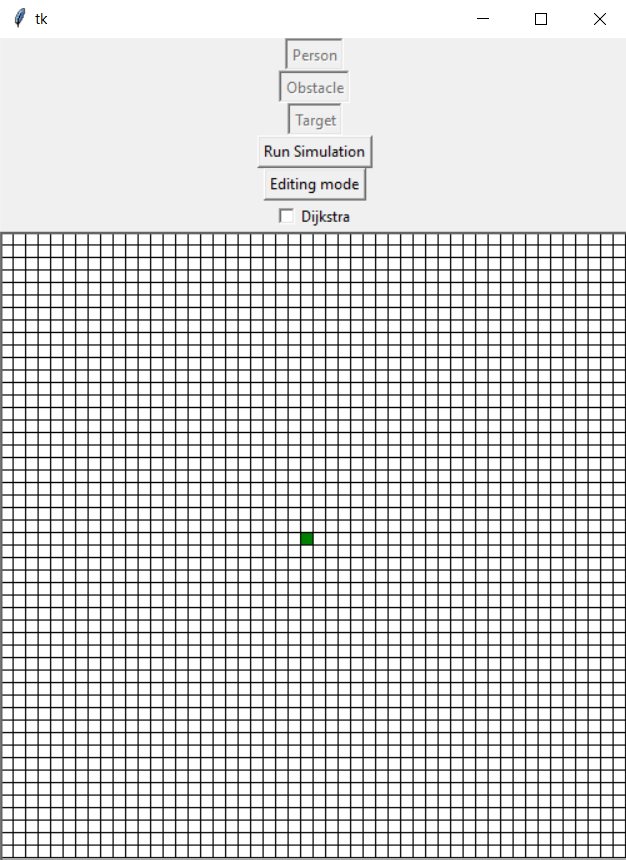
\includegraphics[width=0.3\textwidth]{task3_3.png}\label{fig:task3-3}}
    \caption{Screenshots showing 3 different stages of the task 3. The sub-figure (a) shows the initial setup; sub-figure (b) shows the environment in the middle of the simulation; sub-figure (c) shows the end on the simulation, when all pedestrians reached the target and have been absorbed.}
    \label{fig:task3}
\end{figure}
\end{task}


\begin{task}{4, Obstacle avoidance}
\paragraph{No obstacle avoidance}
Without any kind of obstacle avoidance implemented, the pedestrians will consider other pedestrians and obstacles as blank cells, therefore it is inevitable that they step on one another and that obstacles are unable to act as barriers.\\
For example, in the case depicted in Figure 10 of \cite{RiMEA}, i.e. a bottleneck situation, the pedestrians would just step on the obstacle and other pedestrians as they were not there at all, so they would not pass through the bottleneck, but simply go straight towards the target.

\paragraph{Rudimentary obstacle avoidance}
The \textit{rudimentary obstacle avoidance} mechanism implemented in this project consists of making the pedestrians simply not step on other pedestrians or obstacles.\\
This is accomplished through a \textbf{cost matrix}.
In this first, simpler implementation, pedestrians simply try to reach the target moving towards its direction.
Every pedestrian, before planning the move, builds its own cost matrix, which is a matrix with the same size of the grid and where every item represents a cell.
The cost placed in every cell is simply the \textit{euclidean distance} between the target and the cell in object.
At this point the agent, when planning the move, chooses the neighbor cell with the lowest cost.
Before this, though, a post-processing of the cost matrix is necessary: all the cells occupied (or that will be occupied
\footnote{Since pedestrians decide where to move in turns, when one is computing its cost matrix, it already knows where the pedestrian that planned the move before it are going to be when it is going to actually move.}
) by other pedestrians or obstacles will have their cost set to infinity.\\
Concerning the \textit{chicken test}
\footnote{There is one pedestrian in front of a target, but some obstacles are placed in between them acting as a cage/trap for the pedestrian.}
instead, with this kind of obstacle avoidance, the pedestrian (depicted in red) will start walking towards the target (depicted in green) until it gets trapped by the obstacles (depicted in black) and at this point it will stay there until the simulation ends.
\hyperref[fig:chicken]{Figure \ref{fig:chicken}.a} shows the initial setup of the chicken test, while \hyperref[fig:chicken]{Figure \ref{fig:chicken}.b} shows how the simulation ends with the pedestrian stuck in the trap.

\begin{figure}[H]
    \centering
    \subfloat[a]{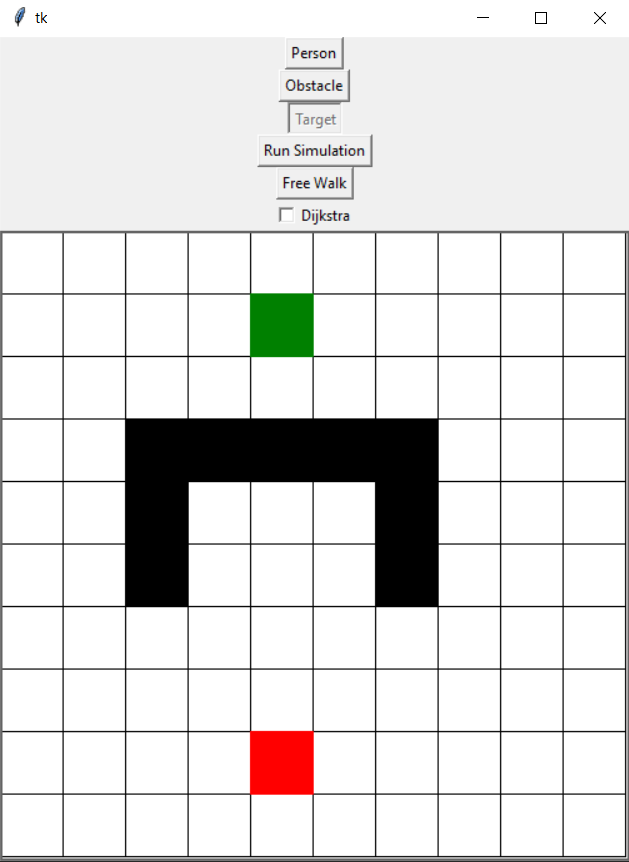
\includegraphics[width=0.4\textwidth]{chicken_test_1.png}\label{fig:chicken-1}}
    \subfloat[b]{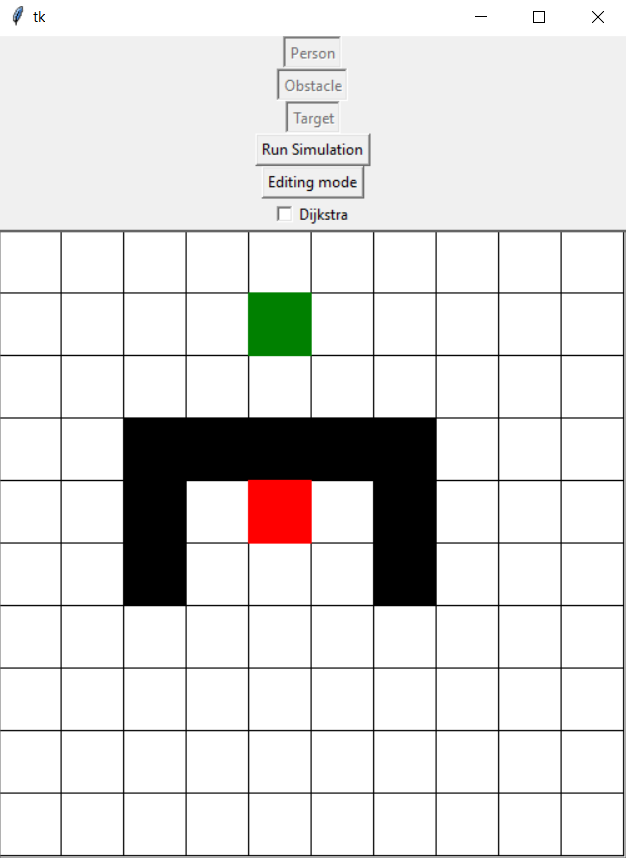
\includegraphics[width=0.4\textwidth]{chicken_test_2.png}\label{fig:chicken-2}}
    \caption{Screenshots showing respectively: (a) the initial setup of the chicken test; (b) the pedestrian stuck in the trap at the end of the simulation.}
    \label{fig:chicken}
\end{figure}

\paragraph{Dijkstra's algorithm}
To overcome the problems highlighted in the \textit{"chicken test"}, the Dijkstra's algorithm can be a viable solution.\\
Its purpose is to find the shortest (less costly) path between 2 nodes in a graph.
In the current case it is possible to consider each cell as a vertex with undirected archs connecting it to and only to its neighbor cells.
Dijkstra starts from a source cell, i.e. the pedestrian which is calculating the cost matrix, and tries to reach a destination cell (i.e. the target) by iteratively visiting the neighbors of the current cell in object and updating the overall cost to reach that neighbor from the source passing from a certain cell as second-last one in the path.\\
In this case, the \textit{"chicken test"} is completed successfully, as show in \hyperref[fig:chicken-dijkstra]{Figure \ref{fig:chicken-dijkstra}}, the red pedestrian is able to go around the U-shaped obstacle.\\\\
Note: on the graphical interface, to run a certain simulation using the Dijkstra's algorithm to compute the best path, it is necessary to select the apposite checkbox, otherwise the simulation will be run with a more rudimentary obstacle avoidance policy (explained in the previous paragraph) where the next cell in the path is selected 

\begin{figure}[H]
    \centering
    \subfloat[a]{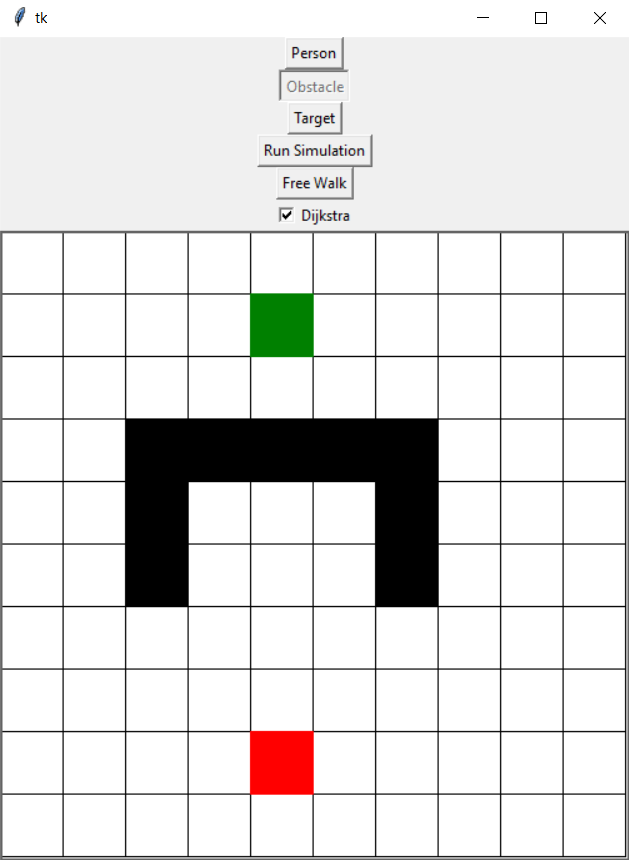
\includegraphics[width=0.3\textwidth]{chicken_test_dijkstra_1.png}\label{fig:chicken-dijkstra-1}}
    \hfill
    \subfloat[b]{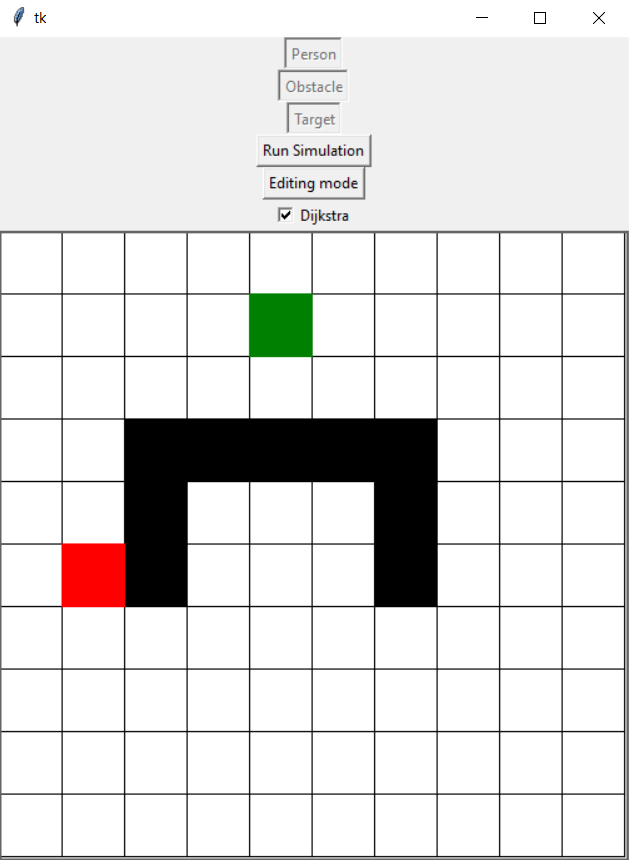
\includegraphics[width=0.3\textwidth]{chicken_test_dijkstra_2.png}\label{fig:chicken-dijkstra-2}}
    \hfill
    \subfloat[c]{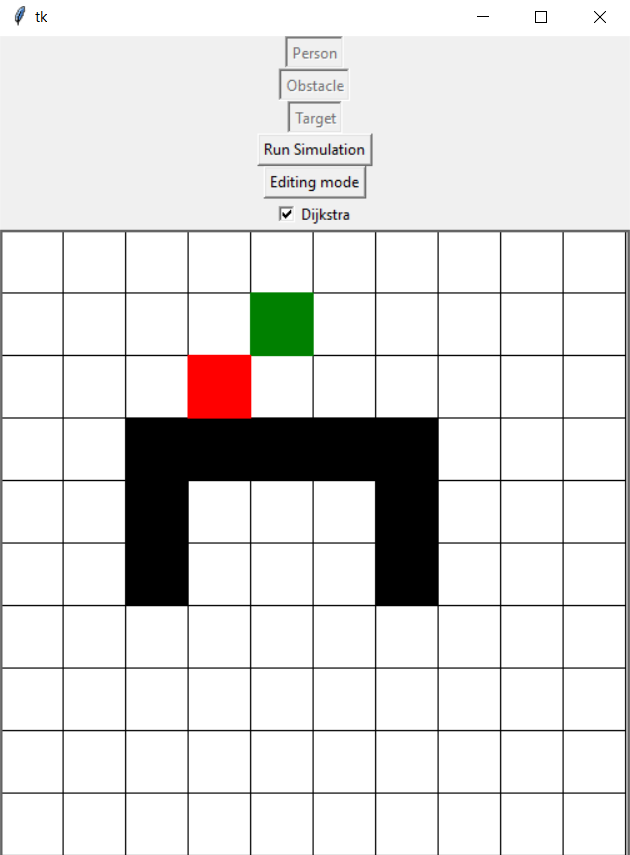
\includegraphics[width=0.3\textwidth]{chicken_test_dijkstra_3.png}\label{fig:chicken-dijkstra-3}}
    \caption{Screenshots showing 3 different stages of the \textit{"chicken test"} executed with the Dijkstra's algorithm. The sub-figure (a) shows the initial setup; sub-figure (b) shows the environment in the middle of the simulation; sub-figure (c) shows the environment when near the end on the simulation.}
    \label{fig:chicken-dijkstra}
\end{figure}

Another interesting experiment which can be carried on is about the \textit{bottleneck test}. Both the \textit{rudimentary obstacle avoidance} and the more sophisticated \textit{Dijkstra implementation} can achieve reaching the objective. The interesting part stands in how they reach it. In fact, looking at \textbf{\hyperref[fig:bottleneck-no-dijkstra]{Figure \ref{fig:bottleneck-no-dijkstra}}} one can appreciate how all the Pedestrians try to reach the upper right corner of the leftmost part of the bottleneck, since that cell is the \textit{nearest} to the target (talking Euclidean Distance) before going into the small corridor. On the other hand, looking at \textbf{\hyperref[fig:bottleneck-dijkstra]{Figure \ref{fig:bottleneck-dijkstra}}}, the algorithm makes it so that the optimal path is promptly found, making all the Pedestrians form a nice queue without moving to unnecessary cells.

\begin{figure}[H]
    \centering
    \subfloat[a]{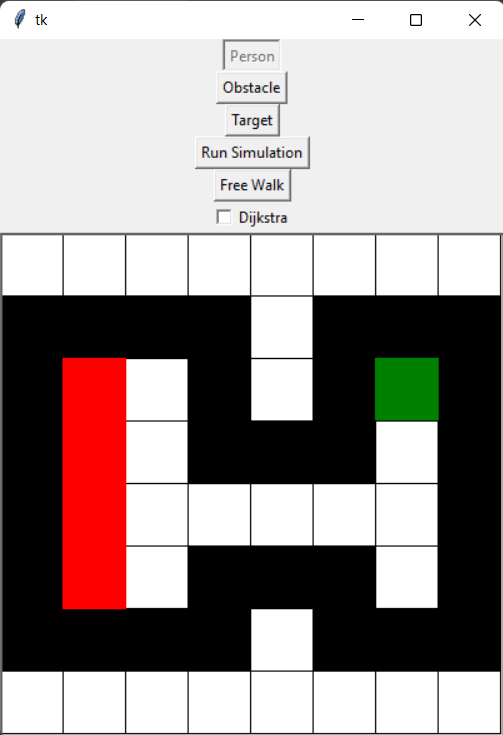
\includegraphics[width=0.3\textwidth]{bottleneck_no_d_1.png}\label{fig:bottleneck-no-d-1}}
    \hfill
    \subfloat[b]{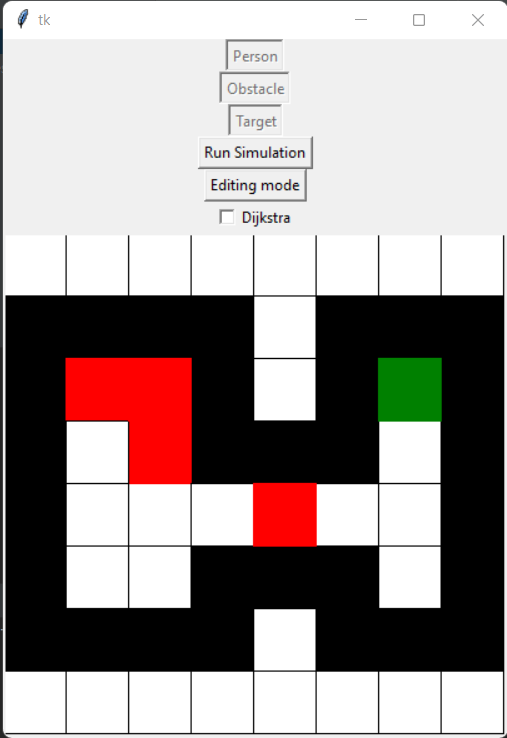
\includegraphics[width=0.3\textwidth]{bottleneck_no_d_2.png}\label{fig:bottleneck-no-d-2}}
    \hfill
    \subfloat[c]{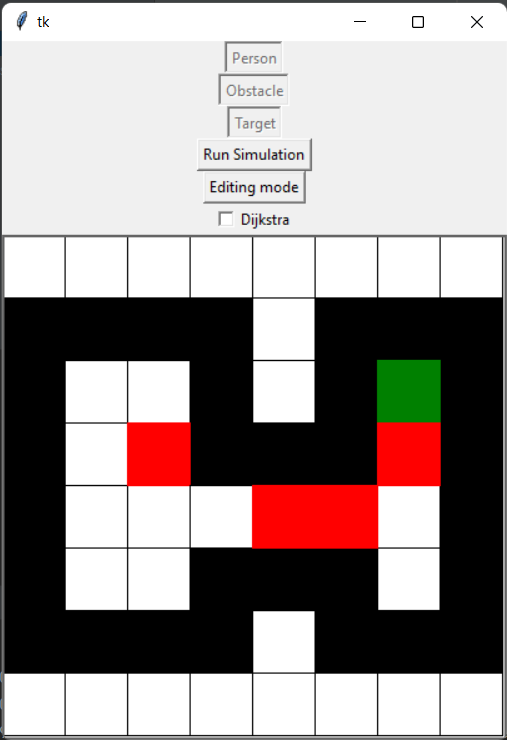
\includegraphics[width=0.3\textwidth]{bottleneck_no_d_3.png}\label{fig:bottleneck-no-d-3}}
    \caption{Screenshots showing 3 different stages of the \textit{"bottleneck test"} executed \textbf{without} the Dijkstra's algorithm. The sub-figure (a) shows the initial setup; sub-figure (b) shows the environment in the middle of the simulation; sub-figure (c) shows the environment when near the end on the simulation.}
    \label{fig:bottleneck-no-dijkstra}
\end{figure}

\begin{figure}[H]
    \centering
    \subfloat[a]{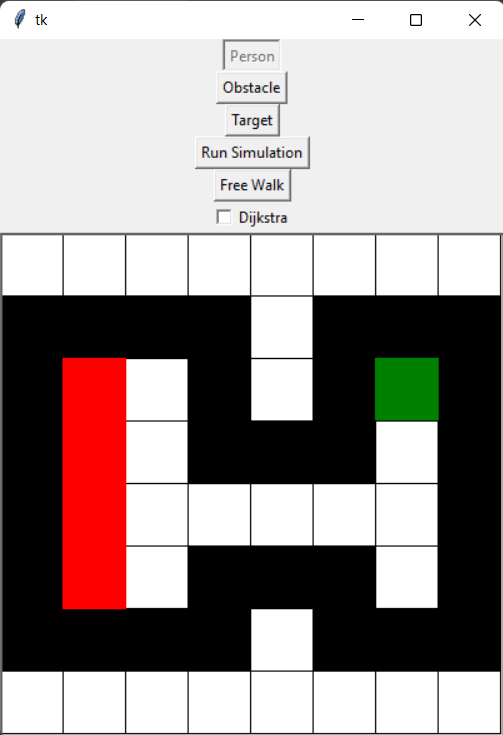
\includegraphics[width=0.3\textwidth]{bottleneck_no_d_1.png}\label{fig:bottleneck-1}}
    \hfill
    \subfloat[b]{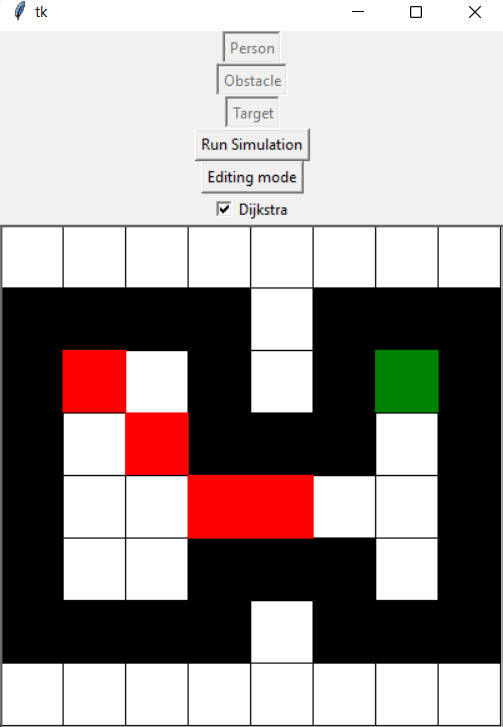
\includegraphics[width=0.3\textwidth]{bottleneck_2.png}\label{fig:bottleneck-2}}
    \hfill
    \subfloat[c]{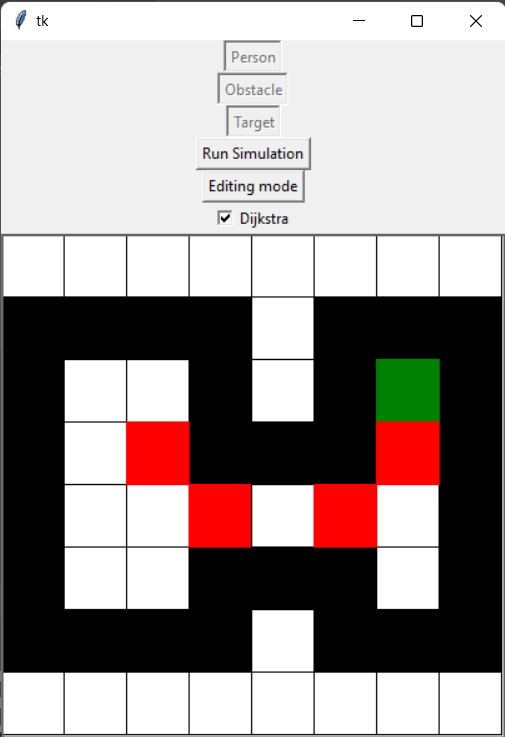
\includegraphics[width=0.3\textwidth]{bottleneck_3.png}\label{fig:bottleneck-3}}
    \caption{Screenshots showing 3 different stages of the \textit{"bottleneck test"} executed \textbf{with} the Dijkstra's algorithm. The sub-figure (a) shows the initial setup; sub-figure (b) shows the environment in the middle of the simulation; sub-figure (c) shows the environment when near the end on the simulation.}
    \label{fig:bottleneck-dijkstra}
\end{figure}

\end{task}




\begin{task}{5, Tests}
The RiMEA \cite{RiMEA} benchmark is used to validate the implementation of the pedestrians' behavior.

\paragraph{TEST 1 - RiMEA scenario 1: straight line}
There is a pedestrian on one end a corridor (delimited by obstacles) and a target on the other end (\hyperref[fig:rimea1]{Figure \ref{fig:rimea1}.a}).\\
Each cell is $1m^2$ and the pedestrian's size is such to fill exactly 1 cell, furthermore the walking speed is 1m/s.
The corridor is 2 meters wide and 40 meters long, so the pedestrian has to make 39 steps to reach the target.\\\\
In the experiments it is shown that the time of the simulation is exactly \textbf{39.0s} and the pedestrian's speed is \textbf{1.0m/s}.\\\\
\hyperref[fig:rimea1]{Figure \ref{fig:rimea1}} illustrates 3 moments of the simulation.

\begin{figure}[H]
    \centering
    \subfloat[a]{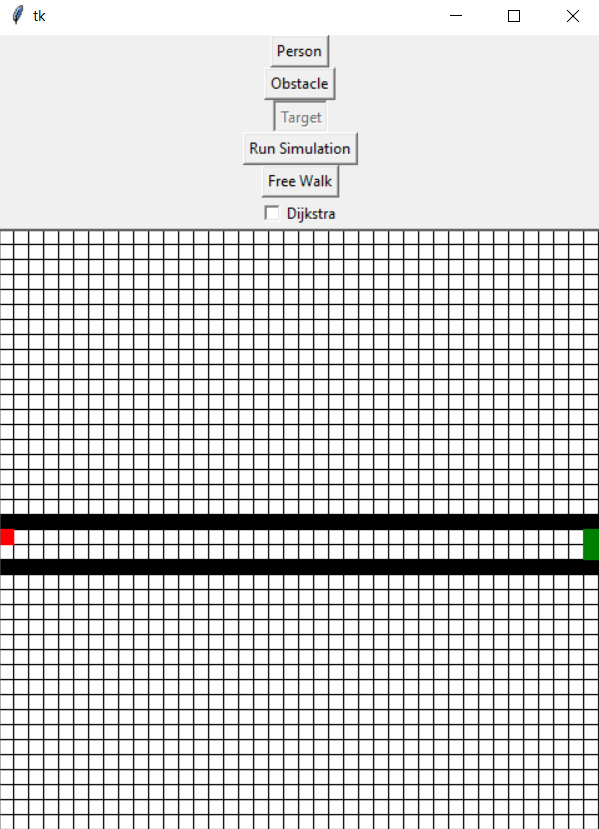
\includegraphics[width=0.28\textwidth]{rimea1_1.png}\label{fig:rimea1-1}}
    \hfill
    \subfloat[b]{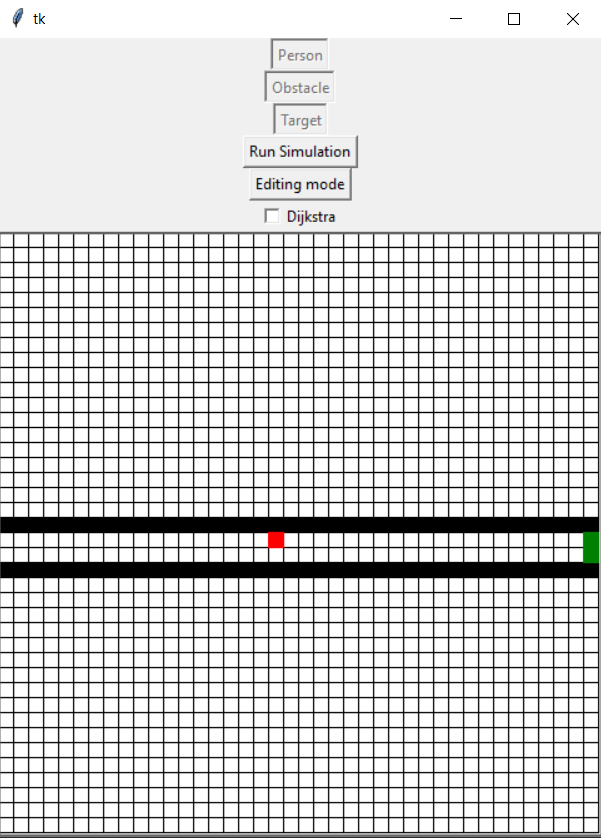
\includegraphics[width=0.28\textwidth]{rimea1_2.png}\label{fig:rimea1-2}}
    \hfill
    \subfloat[c]{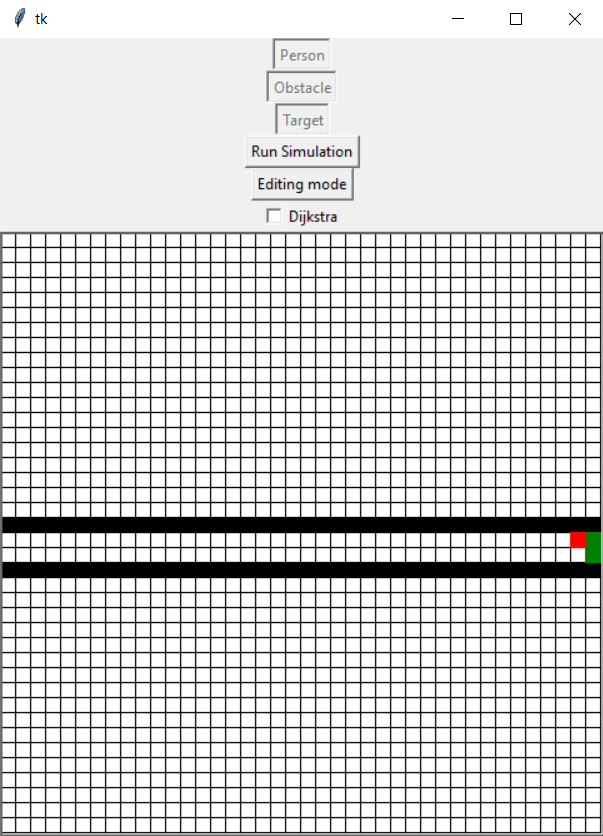
\includegraphics[width=0.28\textwidth]{rimea1_3.png}\label{fig:rimea1-3}}
    \caption{Screenshots showing 3 different stages of the RiMEA scenario 1. The sub-figure (a) shows the initial setup; sub-figure (b) shows the environment in the middle of the simulation; sub-figure (c) shows the environment when near the end on the simulation.}
    \label{fig:rimea1}
\end{figure}
\pagebreak
\paragraph{TEST 2 - RiMEA scenario 4: fundamental diagram}\\

This scenario proved to be the most difficult to face, bringing changes to the proposed code and the decision of coming to terms with the request. \\
The original task requires a corridor 1000m long and 10m wide, with three different measuring zones of 2x2m. The proposed implementation does unfortunately fall short on the full requirements. In fact, having such a large number of cells and pedestrians proves to make the simulation unfeasible, with the application freezing and being extremely slow.\\
A few approximations or premises were therefore applied to still provide a viable simulation which respects as much as possible the scenario goals: the implementated scenario shows a grid of 80x80 elements, with a corridor of 9x80 cells. Targets are put on the right end and the corridor is flooded with a density of 0.5$\frac{P}{m^2}$ in a spawning area of 693 cells (produced Pedestrians are 346). Three measuring zones of 3x3m are placed in the left, center and right part of the corridor (measuring zones are colored in \textit{yellow}, as can be appreciated in \textbf{\hyperref[fig:rimea4]{ Figure \ref{fig:rimea4}}}).

\vspace{1cm}


\begin{figure}[h!]
\centering
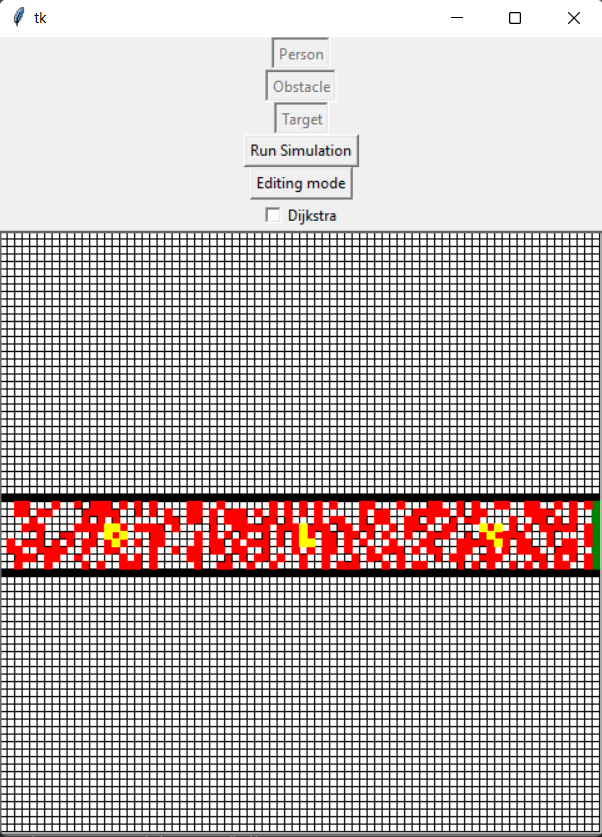
\includegraphics[width=.3\textwidth]{task_5_rimea_4_1.png}\quad
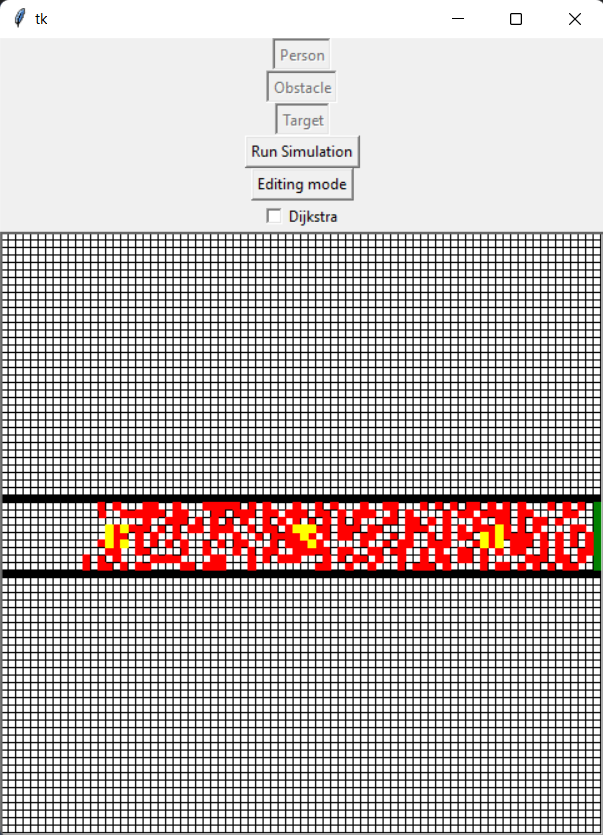
\includegraphics[width=.3\textwidth]{task_5_rimea_4_2.png}\quad
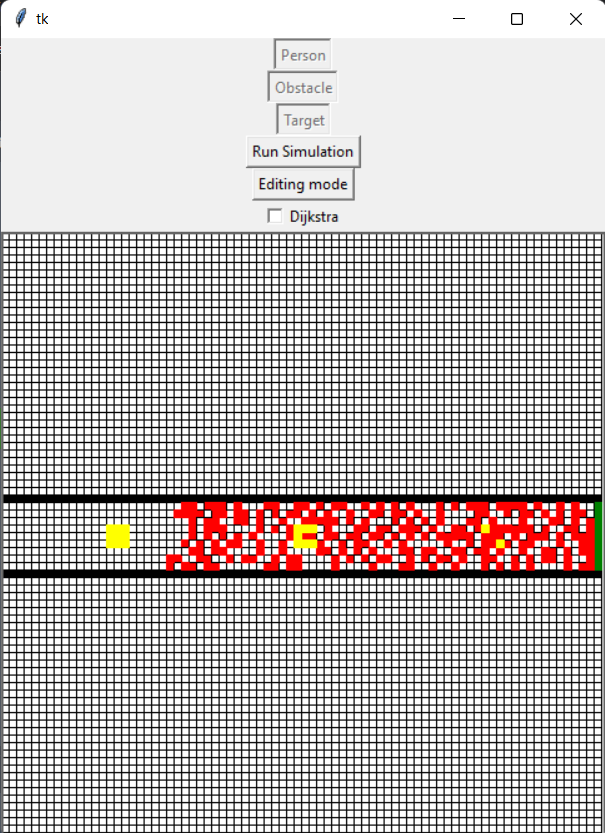
\includegraphics[width=.3\textwidth]{task_5_rimea_4_3.png}

\medskip

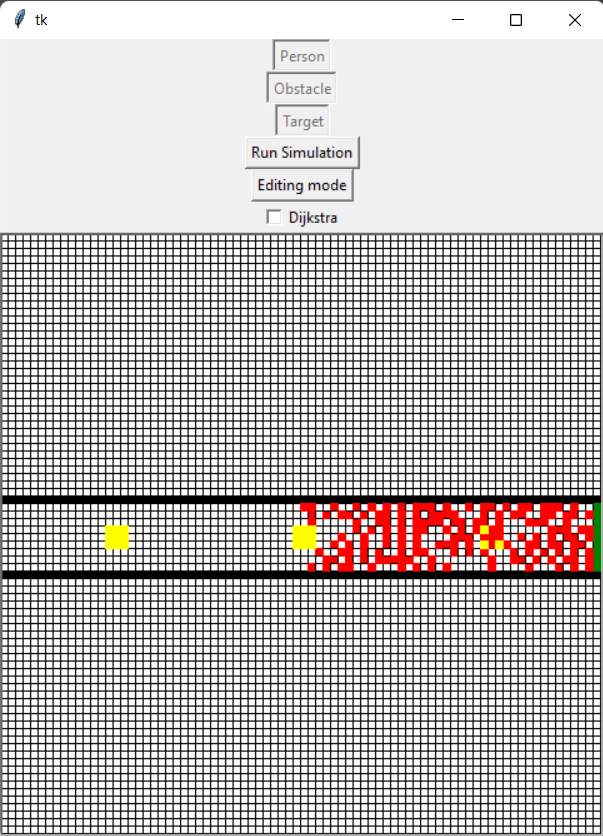
\includegraphics[width=.3\textwidth]{task_5_rimea_4_4.png}\quad
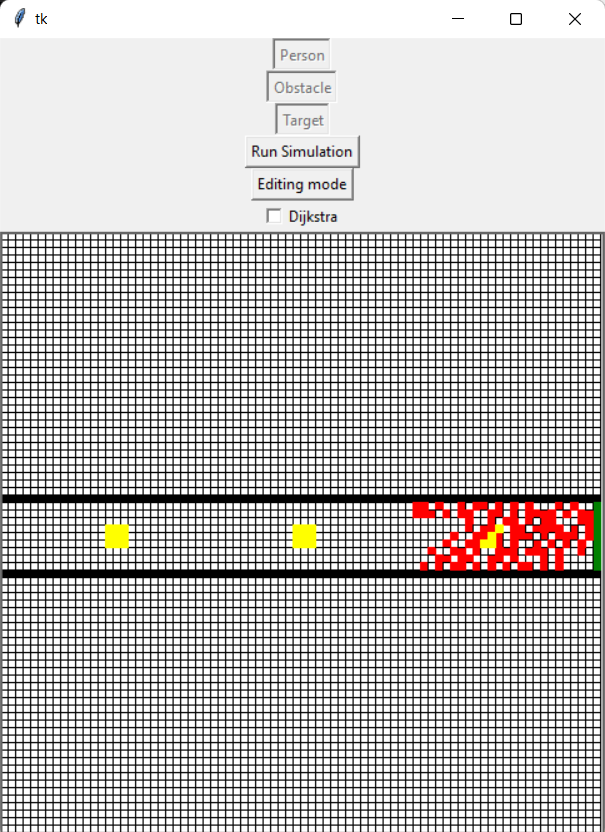
\includegraphics[width=.3\textwidth]{task_5_rimea_4_5.png}\quad
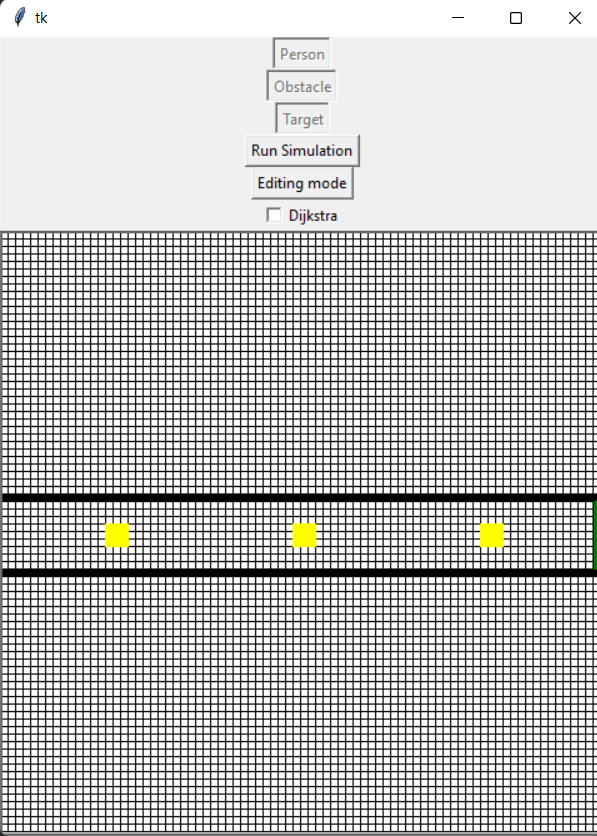
\includegraphics[width=.3\textwidth]{task_5_rimea_4_6.png} 

\caption{\centering Screenshots showing 6 different stages of the RiMEA scenario 4. Detection zones are in yellow and the figures show how they remain empty after all pedestrians have passed by.  }
\label{fig:rimea4}
\end{figure}

To fulfill the requirements a new object and its interaction with the environment had to be created: the \textit{DetectionZone}, which keeps track of density at each time step as well as speed of travelling pedestrians for a single measuring zone. Once all the pedestrians have reached a target the average metrics over the three measuring zones are combined. 

One can guess another approximation that once again unfortunately follows such a scenario: an approximation on density. In fact, as can be appreciated in \textbf{\hyperref[fig:rimea4]{ Figure \ref{fig:rimea4}}} for the left measuring zone, that zone will have a lot of \textit{zeroed} densities due to the fact of all the pedestrians already having gone past the measuring zone. To avoid lowering too much the final average density (the original purpose would be to have a continual flow of people in the corridor) the trailing zeros in the density vector are trimmed.

Finally, after explaining all the approximations and premises, the result of the experiment shown in \textbf{\hyperref[fig:rimea4]{ Figure \ref{fig:rimea4}}} are:
\begin{itemize}
    \item \textit{Average Density:} 0.25
    \item \textit{Average Speed:} 1.0
    \item \textit{Average Flow:} 0.25
\end{itemize}
The \textit{average speed} value was expected, since the speed of each Pedestrian is fixed to being 1.0. The amount of times a person stands still is negligible in this case since using the \textit{rudimentary obstacle avoidance} makes it so that a Pedestrian stands still only in the case it is surrounded by obstacles/other Pedestrians.

The \textit{average density} is instead not what one would expect (and therefore an analogous discussion can be done for the \textit{average flow}). The expected value was of 0.5, the original density. The difference can be motivated by both the approximation for passive measuring zones and by the Pedestrians changing direction and going above/below the measuring zone.

\paragraph{TEST 3 - RiMEA scenario 6: movement around a corner}
The RiMEA scenario 6 consists of having 20 pedestrians moving around a left corner to reach a target placed on the end of it.
The goal is to successfully go around without passing through walls.\\
This can be accomplished both with the \textit{"rudimentary obstacle avoidance mechanism"} and with the \textit{Dijkstra's algorithm}.\\\\
In the first case, illustrated in \hyperref[fig:rimea6-no-dijkstra]{Figure \ref{fig:rimea6-no-dijkstra}}, the movements of the pedestrians are less precise and more "short-sighted".
It is to be expected, since the only measure they are considering in order to decide where to go is the euclidean distance between the candidate destination cell and the target (of course the candidate destination cell must be empty).\\\\
With the Dijkstra's algorithm (\hyperref[fig:rimea6-dijkstra]{Figure \ref{fig:rimea6-dijkstra}}), instead, the pedestrians tend to concentrate on the best path.
Again, this is an expected behavior, since every pedestrian calculates the best path for itself and tries to stick to it as much as possible, with exceptions in case some cells are occupied by other pedestrians in a certain moment.
It is possible to notice in \hyperref[fig:rimea6-dijkstra]{Figure \ref{fig:rimea6-dijkstra}(c)} that the furthest pedestrians on the outside of the optimal path could try to pass around the the crowd, but this would be true in a real-life situation.
In the proposed case every pedestrian computes its optimal path regardless of the others, simply taking into consideration the obstacles and the targets, thus explained why they don't seem to take "alternative" routes. They find the best path, which might be blocked by other pedestrians, therefore they wait. They are extremely polite pedestrians.

\begin{figure}[H]
    \centering
    \subfloat[a]{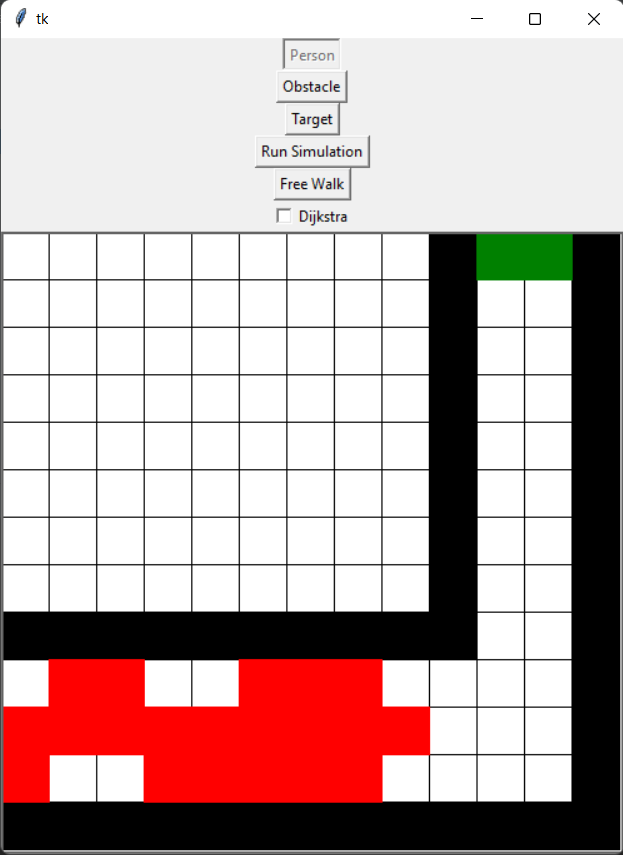
\includegraphics[width=0.3\textwidth]{rimea6_1_no_d.png}\label{fig:rimea6-1-no-dijkstra}}
    \hfill
    \subfloat[b]{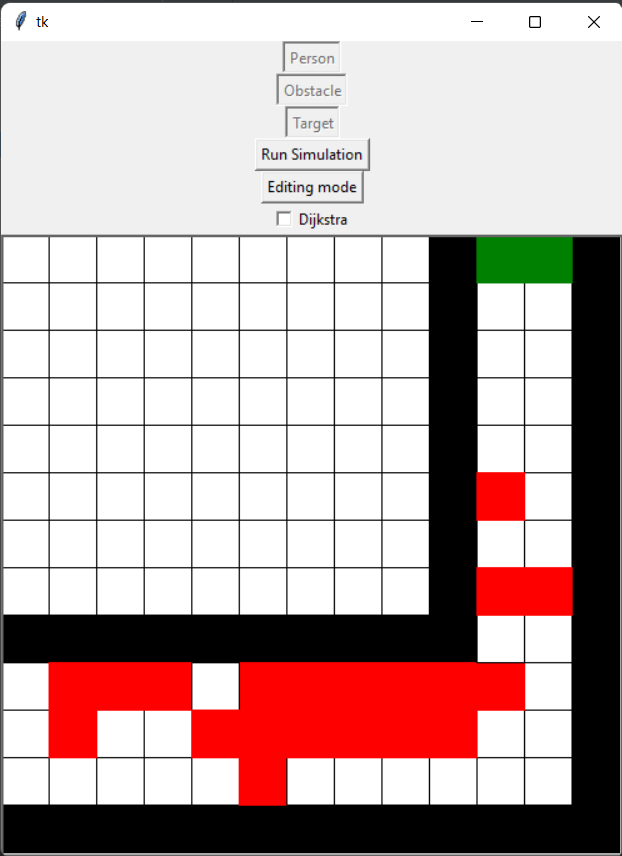
\includegraphics[width=0.3\textwidth]{rimea6_2_no_d.png}\label{fig:rimea6-2-no-dijkstra}}
    \hfill
    \subfloat[c]{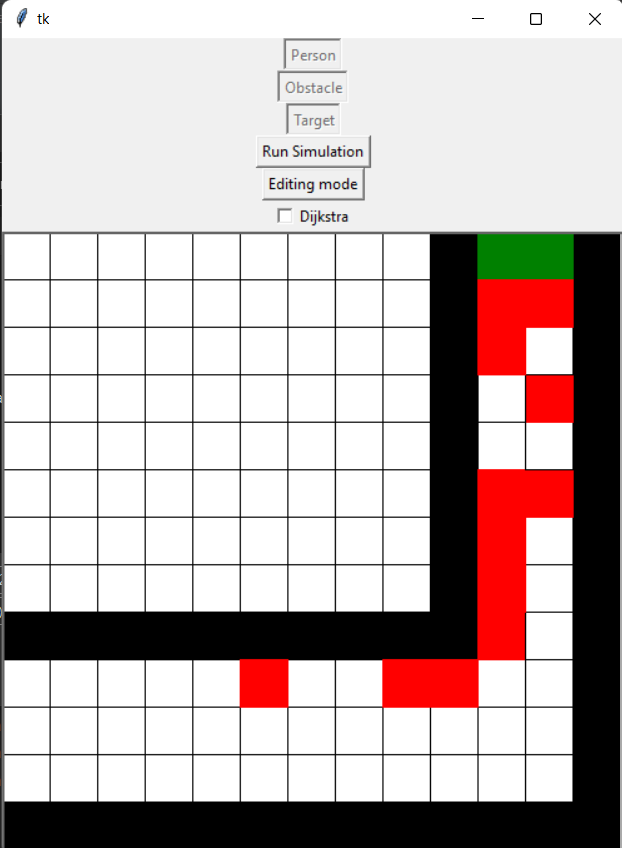
\includegraphics[width=0.3\textwidth]{rimea6_3_no_d.png}\label{fig:rimea6-3-no-dijkstra}}
    \caption{}
    \label{fig:rimea6-no-dijkstra}
\end{figure}

\begin{figure}[H]
    \centering
    \subfloat[a]{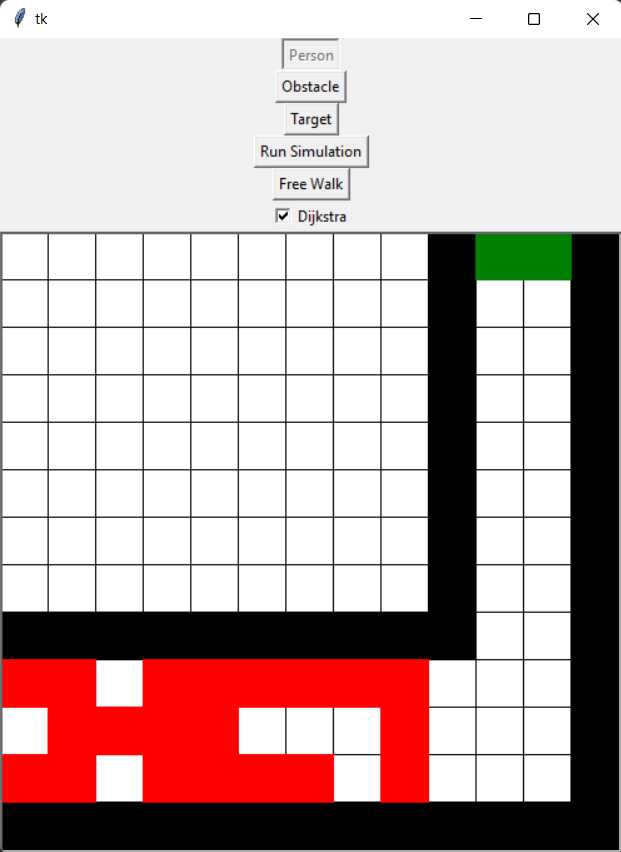
\includegraphics[width=0.3\textwidth]{rimea6_1.png}\label{fig:rimea6-1}}
    \hfill
    \subfloat[b]{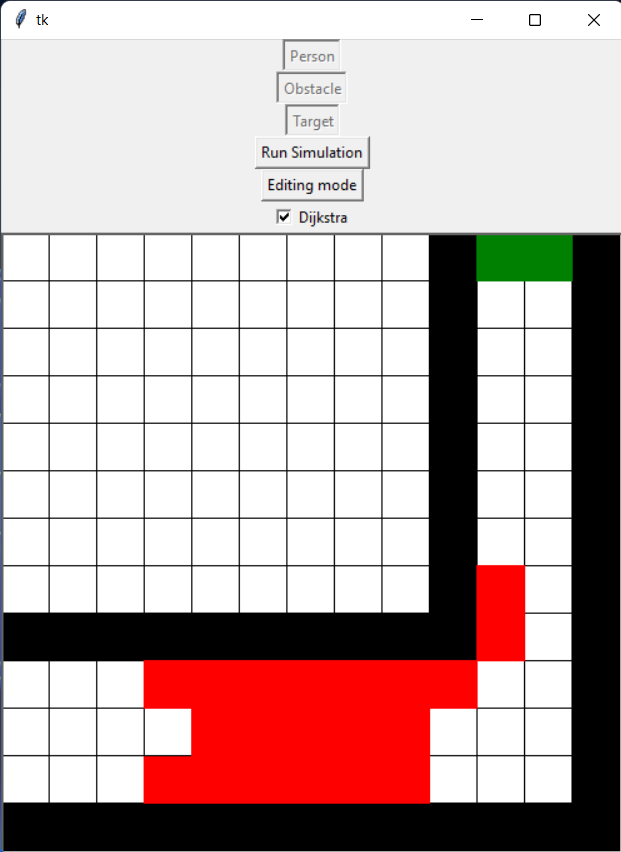
\includegraphics[width=0.3\textwidth]{rimea6_2.png}\label{fig:rimea6-2}}
    \hfill
    \subfloat[c]{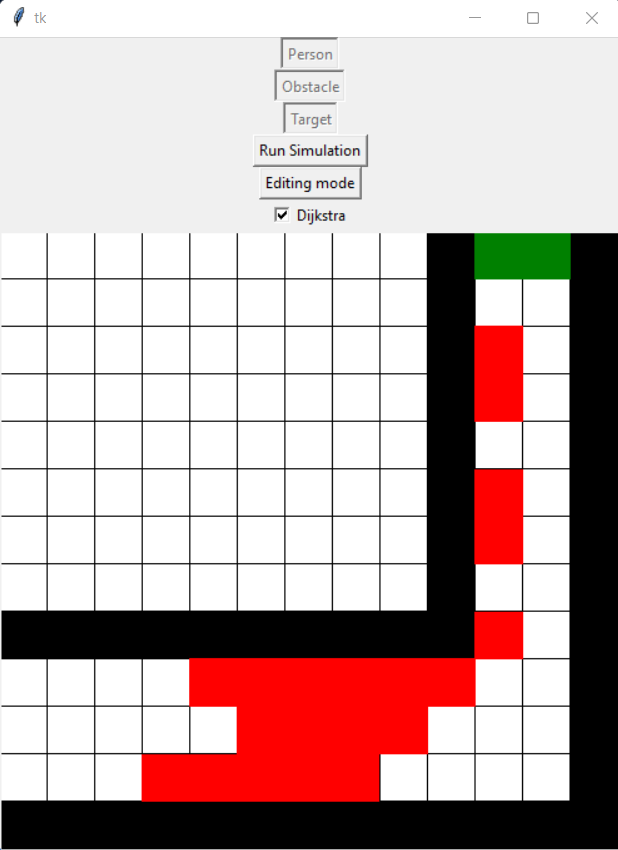
\includegraphics[width=0.3\textwidth]{rimea6_3.png}\label{fig:rimea6-3}}
    \caption{}
    \label{fig:rimea6-dijkstra}
\end{figure}

\paragraph{TEST 4 - RiMEA scenario 7: demographic parameters}
The RiMEA scenario 7 focuses on having different walking speeds for different pedestrians depending on their demographics.\\
The various speeds are sampled from a specific interval that depends on the age of the subject, the minimum of which is 3 years old and the maximum is 80.
The minimum and maximum speed for every age interval is organized as follows:
\begin{itemize}
    \item 3-10 years old: speed $\in[0.6, 1.2)$ m/s
    \item 11-20 years old: speed $\in[1.2, 1.6)$ m/s
    \item 21-50 years old: speed $\in[1.4, 1.6)$ m/s
    \item 51-70 years old: speed $\in[1.1, 1.4)$ m/s
    \item 71-80 years old: speed $\in[0.7, 1.1)$ m/s
\end{itemize}
The proposed ranges are derived by heuristically approximating Figure 2 from RiMEA \cite{RiMEA} benchmark as a piecewise function.

The scenario execution calls for a method for sampling the speed of 50 Pedestrians (\texttt{utils.sample\_age\_speed}) and initializes a 50x50m grid where all Pedestrians are put on the far left and targets on the far right. The objective is to observe the respecting of the pedestrians injected velocity by measuring it. The proposed execution makes this goal both visually and statistically easy to achieve, in fact all is needed is the time for reaching the target and the space travelled.

A visual understanding of the executions can be appreciated in \textbf{\hyperref[fig:rimea7]{ Figure \ref{fig:rimea7}}}, where there are faster red dots and slower ones, probably referring to old people or little kids.

\begin{figure}[H]
    \centering
    \subfloat[a]{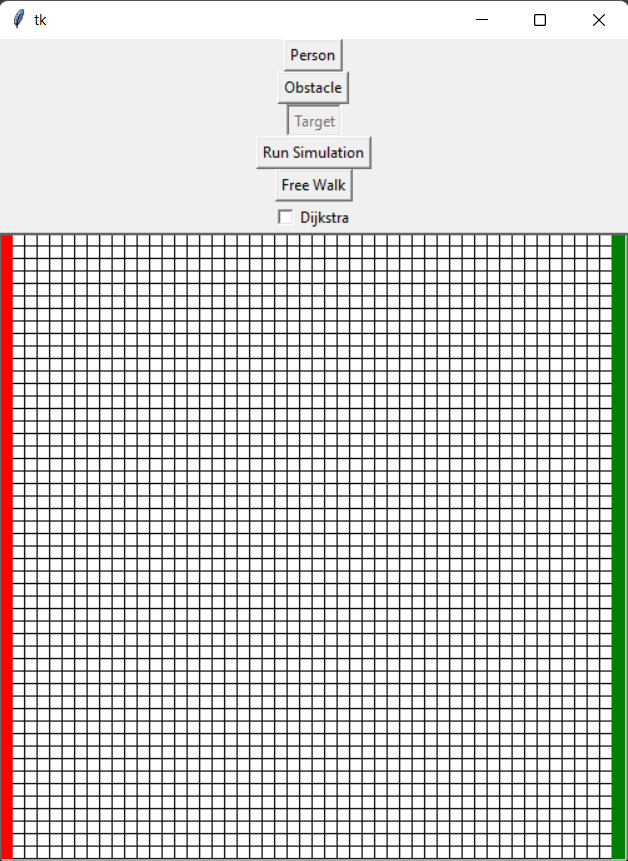
\includegraphics[width=0.3\textwidth]{rimea7_1.png}\label{fig:rimea7-1}}
    \hfill
    \subfloat[b]{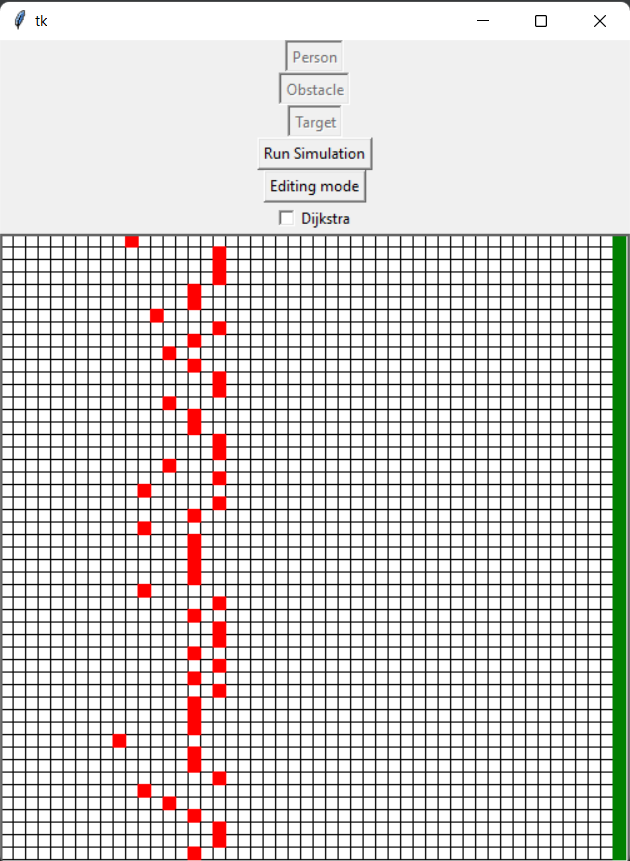
\includegraphics[width=0.3\textwidth]{rimea7_2.png}\label{fig:rimea7-2}}
    \hfill
    \subfloat[c]{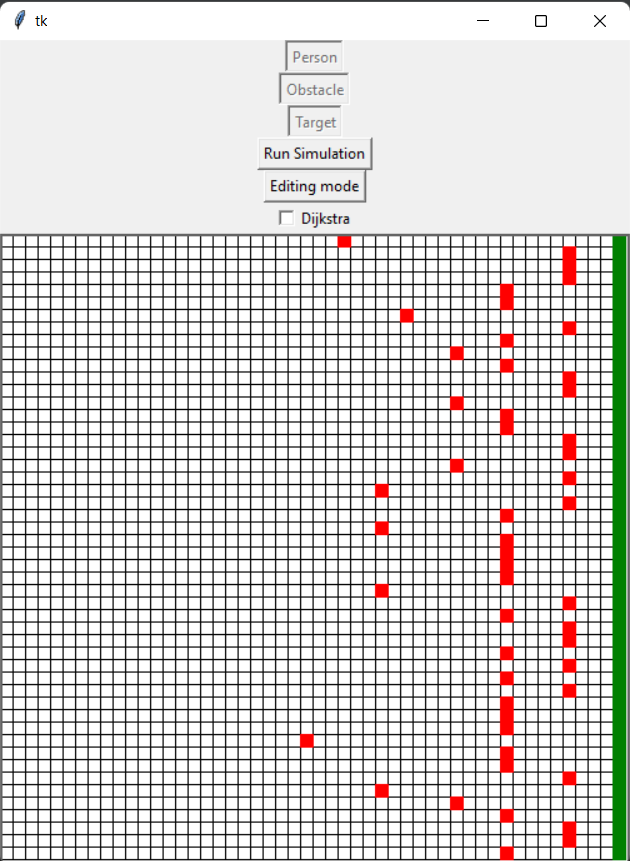
\includegraphics[width=0.3\textwidth]{rimea7_3.png}\label{fig:rimea7-3}}
    \caption{}
    \label{fig:rimea7}
\end{figure}

It is important to remark that the cellular automata execution is not parallel, but sequential. In particular a graphical update happens after all the Pedestrians have had the chance of planning/executing a move (the Pedestrian choosing order is randomized to preserve equality) and, moreover, between two graphical updates a call to \texttt{sleep} is made to simulate the passing of a time step. This preamble is fundamental to understand the discretization of time, leading to small differences between the \textit{expected speed} for a Pedestrian and the \textit{measured speed}. It is anyway interesting to notice that the discrepancy will be proportional to the time step chosen (in the case of \textbf{\hyperref[fig:rimea7]{Figure \ref{fig:rimea7}}} is 0.1s). Results for the 50 Pedestrians are shown in \textbf{\hyperref[tb:rimea7]{Table \ref{tb:rimea7}}}, highlighting what just discussed. At the end of the table also a comparison between the \textit{average measured speed} and \textit{average expected speed}. It is noticeable how the speeds are respected, with the errors being below the threshold imposed by the time step.

This subtask asked for the implementation of the possibility of having Pedestrians with different speeds, a feature not present beforehand. This new ability was included by adding a new field to the Pedestrian constructor and managing the traversing of cells in a timely correct behaviour (dividing the waiting time for movement by the Pedestrian cell).

\begin{table}[ht!]
    	    \centering
    	    \small
    	    \begin{tabular}{ |c|c|c|c| }
            \hline
            \textbf{pedestrian} & \textbf{time taken} & \textbf{measured speed} & \textbf{expected speed}\\
            \hline
            Pedestrian 1  & 34.50 & 1.43 & 1.55\\
            Pedestrian 2  & 34.50 & 1.43 & 1.56\\
            Pedestrian 3  & 34.50 & 1.42 & 1.55\\
            Pedestrian 4  & 34.50 & 1.43 & 1.58\\
            Pedestrian 5  & 34.60 & 1.43 & 1.42\\
            Pedestrian 6  & 34.60 & 1.43 & 1.54\\
            Pedestrian 7  & 34.60 & 1.43 & 1.47\\
            Pedestrian 8  & 34.60 & 1.43 & 1.52\\
            Pedestrian 9  & 34.60 & 1.43 & 1.43\\
            Pedestrian 10 & 34.60 & 1.43 & 1.48\\
            Pedestrian 11 & 34.60 & 1.43 & 1.49\\
            Pedestrian 12 & 34.60 & 1.43 & 1.42\\
            Pedestrian 13 & 34.60 & 1.43 & 1.52\\
            Pedestrian 14 & 34.60 & 1.43 & 1.51\\
            Pedestrian 15 & 34.60 & 1.43 & 1.42\\
            Pedestrian 16 & 34.60 & 1.43 & 1.54\\
            Pedestrian 17 & 34.60 & 1.43 & 1.48\\
            Pedestrian 18 & 34.60 & 1.43 & 1.51\\
            Pedestrian 19 & 39.40 & 1.25 & 1.4\\
            Pedestrian 20 & 39.40 & 1.25 & 1.4\\
            Pedestrian 21 & 39.50 & 1.25 & 1.3\\
            Pedestrian 22 & 39.50 & 1.25 & 1.28\\
            Pedestrian 23 & 39.50 & 1.25 & 1.38\\
            Pedestrian 24 & 39.50 & 1.25 & 1.33\\
            Pedestrian 25 & 39.50 & 1.25 & 1.39\\
            Pedestrian 26 & 39.50 & 1.25 & 1.33\\
            Pedestrian 27 & 39.50 & 1.25 & 1.29\\
            Pedestrian 28 & 39.50 & 1.25 & 1.3\\
            Pedestrian 29 & 39.50 & 1.25 & 1.39\\
            Pedestrian 30 & 39.50 & 1.25 & 1.31\\
            Pedestrian 31 & 39.50 & 1.25 & 1.41\\
            Pedestrian 32 & 39.50 & 1.25 & 1.37\\
            Pedestrian 33 & 39.50 & 1.25 & 1.27\\
            Pedestrian 34 & 39.50 & 1.25 & 1.3\\
            Pedestrian 35 & 39.50 & 1.25 & 1.27\\
            Pedestrian 36 & 39.50 & 1.25 & 1.37\\
            Pedestrian 37 & 39.50 & 1.25 & 1.38\\
            Pedestrian 38 & 39.50 & 1.25 & 1.34\\
            Pedestrian 39 & 39.50 & 1.35 & 1.37\\
            Pedestrian 40 & 44.40 & 1.11 & 1.17\\
            Pedestrian 41 & 44.50 & 1.11 & 1.15\\
            Pedestrian 42 & 44.50 & 1.11 & 1.16\\
            Pedestrian 43 & 44.50 & 1.11 & 1.13\\
            Pedestrian 44 & 49.30 & 1.00 & 1.1\\
            Pedestrian 45 & 54.40 & 0.90 & 0.92\\
            Pedestrian 46 & 54.30 & 0.90 & 0.96\\
            Pedestrian 47 & 54.40 & 0.90 & 0.93\\
            Pedestrian 48 & 54.30 & 0.90 & 0.98\\
            Pedestrian 49 & 58.80 & 0.83 & 0.85\\
            Pedestrian 50 & 69.10 & 0.71 & 0.76\\
            \hline
            \textbf{Average Pedestrian} & - & \textbf{1.25} & \textbf{1.32}\\
            \hline
            \end{tabular}
        \caption{RiMEA Test 7 Results}
    	    \label{tb:rimea7}
    \end{table}
\end{task}

\newpage
\bibliographystyle{plain}
\bibliography{references}









\end{document}